%% ConsILR-2026 paper. Generated from paper_template.tex by build_paper.py (numbers come from results/results.json).
%% The same text is converted to the official Word format by build_docx.py.
\documentclass[11pt]{article}
\usepackage{consilr2026}
\usepackage[utf8]{inputenc}
\usepackage[T1]{fontenc}
\usepackage{times}
\usepackage{url}
\usepackage{latexsym}
\usepackage{authblk}
\usepackage{hyperref}
\hypersetup{hidelinks}
\usepackage{etoolbox}
\usepackage{graphicx}
\usepackage{booktabs}
\usepackage{combelow}
\usepackage{newunicodechar}
\newunicodechar{ș}{\cb{s}}
\newunicodechar{ț}{\cb{t}}
\newunicodechar{Ș}{\cb{S}}
\newunicodechar{Ț}{\cb{T}}
\newunicodechar{–}{--}
\newunicodechar{≈}{$\approx$}
\newunicodechar{×}{$\times$}

\renewcommand*{\Authand}{, }
\renewcommand*{\Authands}{, AND }
\renewcommand*{\Affilfont}{\itshape\mdseries}
\setlength{\affilsep}{2em}
\newcommand{\keyword}[1]{\hspace{0.2cm}\fontsize{10}{12}\selectfont\textbf{Keywords: }}
\newcommand{\ro}[1]{\textit{#1}}

\title{\textbf{THE HIDDEN CORE OF ROMANIAN: A GRAPH-THEORETIC ANALYSIS OF DICTIONARY DEFINITIONS}}
\author[1]{VLAD BELCIUG}
\author[1]{ELENA PELICAN}
\affil[1]{``Ovidius'' University of Constanța, Faculty of Mathematics and Informatics,\break Bd. Mamaia 124, Constanța, Romania
\break \texttt{vlad.belciug@365.univ-ovidius.ro, epelican@univ-ovidius.ro}}
\date{}

\begin{document}
\pagestyle{empty}
\maketitle
\thispagestyle{empty}
\begin{abstract}
Dictionary definitions are inherently circular, as words are defined through other words; consequently, a dictionary can only support lexical acquisition if part of its vocabulary is already known. A dictionary represented as a directed graph contains a Kernel, from which all other words can be defined, and minimal grounding sets (MinSets), the smallest sets of words that provide the lexical basis of the entire dictionary. We construct and analyse such a graph for the second edition of the DEX (\ro{Dicționarul explicativ al limbii române}, `The Explanatory Dictionary of the Romanian Language'), comprising <<HW>> headwords. Lemmatisation and headword assignment were performed with a large language model and evaluated against a stronger model and two model-free baselines. The DEX Kernel contains <<K_PCT>> of all headwords and its MinSets <<M_RANGE>>, substantially more than dictionaries of <<X_NLANG>> other languages processed in the same way (MinSets of <<X_M>>). This difference is primarily attributable to reciprocal definitional relations, particularly prevalent in the DEX. Despite its graph-theoretic derivation, the Kernel contains <<SW_K>> of the Romanian equivalents of the Swadesh list and <<G_K>> of Graur's (1954) fundamental lexical stock. These findings suggest that the latent structure of dictionary definitions captures a linguistically meaningful lexical core.
\end{abstract}
\keyword{} lexicography, dictionary graphs, symbol grounding, minimal grounding set, fundamental lexical stock, Romanian, DEX, large language models

\section{Introduction}
A monolingual dictionary explains each word by means of other words. In the DEX, the first sense of \ro{copac} `tree' contains the word \ro{arbore} `tree', and the definition of \ro{arbore} contains \ro{copac}. A reader who knows neither word cannot learn either of them from the dictionary, so some words must be known before the definitions can be used. This is the lexicographic form of the \emph{symbol grounding problem} \cite{harnad1990}. \newcite{blondinmasse2008} and \newcite{picard2013} formulated the problem in terms of graph theory, and \newcite{vincentlamarre2016} measured it on four English dictionaries. They identified in each dictionary a \emph{Kernel} of 7--12\% of the headwords, from which all the other headwords can be defined, and \emph{minimal grounding sets} (MinSets) of about 1\%. A MinSet is a smallest set of words such that, if their meanings are known in advance, every other headword can be learned from definitions alone. Kernel words were also more frequent and acquired earlier by children than the remaining words. The method has since been applied to Spanish \cite{pichardo2017,kostiuk2023} and, through Wiktionary, to six languages including Chinese and Russian \cite{eschrich2024}. It has not been applied to Romanian.

Romanian linguistics has its own tradition of identifying the core of the vocabulary. \newcite{graur1954} selected 1,419 words as the \ro{fondul principal lexical} (fundamental lexical stock) of Romanian, divided them into three groups by degree of certainty and labelled each word with its origin. In a reduced edition he described the selection as subjective \cite{graur1957}, and it was discussed critically at the time \cite{ivanescu1955}. Graur also suggested that the importance of a word is reflected in the space it occupies in dictionaries \cite[pp.~24--25]{graur1954}. Romanian lexicographers have analysed the structure of the lexicographic definition and the requirement that it should not be circular \cite{oprea1976,maranduc2012}, and \newcite{sterian2016} has described definitional deficiencies of the DEX. These studies examine individual definitions. No study has measured circularity over a whole Romanian dictionary.

This paper reports such a measurement for the second edition of the DEX, \ro{Dicționarul explicativ al limbii române} (The Explanatory Dictionary of the Romanian Language; 1996, reprinted 1998)\nocite{dex1998}, in the digitisation of dexonline \cite{dexonline}. We address three research questions. (Q1) How large are the Kernel and the MinSet of the DEX, and how do they compare with those of dictionaries of other languages? (Q2) Which properties of the definitions determine their size? (Q3) Do the Kernel and the MinSet contain the words of independent inventories of basic vocabulary, namely the Swadesh list and Graur's fundamental lexical stock? 

The paper makes five contributions. (1) It gives the first measurement of the latent structure of a Romanian dictionary, computed over all <<HW>> headwords of the DEX. (2) It shows, by processing dictionaries of <<X_NLANG>> other languages with the same procedure, that the DEX is considerably more circular than all of them, and it traces the difference to the reciprocal definition of headwords by synonyms and derivatives. (3) It shows, by comparison with the Swadesh list and with Graur's list, that the Kernel contains the basic vocabulary of Romanian, and that the words used most often in definitions form a distinct group of learned loanwords. (4) It provides a procedure in which a language model resolves ambiguous word forms over a whole dictionary, with an estimate of its reliability and a check that the conclusions do not depend on it; integer programming places the size of the MinSet within an interval of <<GAP1>>. (5) It releases the graph, the computed sets, the list of reciprocally defined pairs and a program that applies the analysis to any dictionary (Section~7).

\section{Background}
\subsection{Dictionaries as Graphs}
Following \newcite{blondinmasse2008}, a dictionary is represented as a directed graph whose vertices are headwords, with an arc $u \rightarrow v$ whenever $u$ occurs in the definition of $v$. A set $U$ of headwords is a \emph{grounding set} if every other headword can be learned from definitions that contain only words of $U$ or words already learned in this way. Formally, $U$ is a grounding set exactly when every directed cycle of the graph contains a vertex of $U$, that is, when $U$ is a \emph{feedback vertex set}. A minimum feedback vertex set is a MinSet. Finding one is NP-hard \cite{karp1972,festa1999}, and a graph usually has many MinSets of the same size. The \emph{Kernel} is obtained by repeatedly deleting the headwords that do not occur in the definition of any remaining headword. Such headwords can always be learned last, so every MinSet lies inside the Kernel. Unlike the MinSet, the Kernel is unique and can be computed in linear time. Its largest strongly connected component, in which every word can be reached from every other word through definitions, is the \emph{Core}; the other components of the Kernel are the \emph{Satellites} \cite{tarjan1972,vincentlamarre2016}.

\subsection{The Fundamental Lexical Stock}
Graur wrote his study in the second half of 1952 \cite{graur1957}, within the framework set by Stalin's 1950 pamphlet on linguistics, which distinguished a stable ``basic word stock'' from the rest of the vocabulary. He adopted, with reservations, criteria proposed in Soviet discussions: a word of the fundamental stock should be used by the whole people, be old and stable, produce derivatives and occur in many fixed expressions. In his view these criteria reduce to the importance of the word in the language \cite{graur1954}. He placed 964 words in the group he considered most certain and 217 and 238 words in two wider groups, and labelled every word with its origin; by his count, 21.49\% of the list is of Slavic origin. Since Graur himself regarded the selection as subjective \cite{graur1957}, we treat his list as a historical expert hypothesis about the core of Romanian vocabulary and compare it with the structure of the dictionary.

\section{Data and Method}
\subsection{The Dictionary}
dexonline \cite{dexonline} distributes under the GNU General Public License the full text of one complete academic dictionary, the second edition of the DEX. In the database dump, the 1998 printing (\ro{DEX '98}) lacks the letters G and H and part of I; these entries are taken from the 1996 printing of the same edition (\ro{DEX '96}). We use DEX '98 and add DEX '96 entries only for headwords absent from DEX '98, which gives <<DEFS>> definitions and <<HW>> distinct headwords. As in \newcite{vincentlamarre2016}, we keep only the first sense of each entry and remove the headword, examples, fixed expressions, abbreviations and etymology, so that only the defining text remains. Homonymous entries with the same spelling are merged into one vertex.

\subsection{From Definitions to Arcs}
Each definition is tokenised, and each token is mapped to the headwords of which it can be an inflected form, using the inflection tables of dexonline (2.27 million forms). Of the <<TOK>> tokens, <<UNK>> cannot be mapped to any headword and are discarded, as in previous work. A further <<AMB>> are ambiguous between two or more headwords: \ro{sare} is the noun \ro{sare} `salt' in the definition of \ro{acid} (\emph{``formează o sare''} `forms a salt') but a form of the verb \ro{sări} `jump' in the definition of \ro{așchie} `splinter' (\emph{``se desprinde sau sare dintr-un material''} `breaks or flies off from a material'), and \ro{fire} may belong to \ro{fir} `thread', \ro{fire} `nature, temper' or \ro{fi} `be'. A wrong assignment adds an arc that does not exist or omits one that does, and either error can create or remove a cycle. The first sense of \ro{copac} illustrates the procedure. It reads \emph{``Plantă cu trunchiul lemnos și înalt, ale cărei crengi se ramifică la o distanță oarecare de sol, formând o coroană; arbore, pom''} (`Plant with a tall woody trunk, whose branches spread out at some distance from the ground, forming a crown; tree, fruit tree') and produces arcs to \ro{copac} from \ro{plantă} `plant', \ro{trunchi} `trunk', \ro{lemnos} `woody', \ro{înalt} `tall', \ro{creangă} `branch', \ro{ramifica} `branch out', \ro{sol} `ground', \ro{coroană} `crown', \ro{arbore} `tree', \ro{pom} `(fruit) tree' and from the function words. The definition of \ro{arbore} contains \ro{copac}, so the two headwords form a cycle of length two, and at least one of them belongs to every grounding set.

\subsection{Resolving Ambiguity with a Language Model}
For each definition that contains ambiguous tokens, a large language model, Claude Haiku~4.5 \cite{anthropic_models}, receives the text of the definition, the ambiguous tokens and, for each token, the candidate headwords with their parts of speech; fifteen definitions are sent in each request. The model answers with the number of the selected candidate. It may select several candidates when the same form occurs with different functions in one definition, and it may answer that no candidate applies, for example for the infinitive marker \ro{a}, which has no entry of its own in the digitised DEX. Language models are increasingly used for annotation tasks of this kind \cite{gilardi2023}. To estimate reliability without human annotators, a stronger model, Claude Opus~5, answered the same questions for 300 randomly sampled definitions. The two models agree on <<AGREE_CONTENT>> of the decisions for content words and on <<AGREE_FUNC>> of those for function words. Most disagreements concern defensible alternatives, such as a participle analysed as an adjective (\ro{declarat} `declared') or as a verb (\ro{declara} `declare'). Agreement between two models does not measure accuracy directly, since both can make the same error. For this reason every measurement is repeated with two procedures that use no language model: assigning each ambiguous form to its most frequent candidate, and linking it to all its candidates. We call the three procedures \emph{regimes}. The complete run with the language model cost about <<COST>> US dollars.

\subsection{Graph Analysis}
The Kernel is computed by iterative deletion and the Core with Tarjan's algorithm, using NetworkX \cite{hagberg2008}. Since the MinSet cannot be computed directly at this scale, we bound its size from both sides. Every grounding set that we construct gives an upper bound. The first is built greedily: vertices without incoming or outgoing arcs, which lie on no cycle, are removed; then the vertex with the largest product of in-degree and out-degree is added to the set and removed from the graph; the two steps are repeated until no cycle remains, and vertices that are not needed are finally removed from the set. Lower bounds come from two sources. A packing of vertex-disjoint cycles gives a lower bound, since each of these cycles requires its own MinSet word. A stronger lower bound comes from the integer linear program that minimises $\sum_v x_v$ subject to $\sum_{v \in c} x_v \geq 1$ for every cycle $c$, with $x_v \in \{0,1\}$, where $x_v = 1$ means that $v$ belongs to the set. We solve it with HiGHS through SciPy \cite{huangfu2018,virtanen2020}. The graph contains too many cycles to list them all, so the constraints are generated iteratively: the program is first solved with all cycles of length two, cycles left unbroken by the solution are added, and the program is solved again. The optimum of each iteration is a valid lower bound. The solution of each iteration is also completed greedily into a grounding set and reduced, which gives a second upper bound; we report the smaller of the two upper bounds.

\subsection{Reference Inventories}
We compare the graph with two inventories of basic vocabulary compiled independently of the DEX. The first is the Swadesh list \cite{swadesh1955}, a list of basic meanings such as `water', `hand', `eat' and `die', used in comparative and historical linguistics because nearly all languages have words for them and these words are seldom borrowed. We use the Romanian equivalents of its 207-item version \cite{wiktionary_swadesh}, which correspond to <<SW_N>> headwords of the DEX. The second inventory is Graur's list, which we transcribed from pages 48--55 of the printed book together with his certainty groups and origin labels. The transcription reproduces his total of 1,419 entries and his Slavic share of 21.49\% exactly. For the three certainty groups we obtain 966, 216 and 237 entries against his 964, 217 and 238, so two of the 1,419 marks remain uncertain. We modernised the orthography according to the 1993 norm (\ro{î} $\rightarrow$ \ro{â} inside words, \ro{sînt} $\rightarrow$ \ro{sunt} `(I/they) am/are') and mapped inflected forms to lemmas (e.g.\ \ro{eram} `(I/we) was/were' and \ro{ești} `(you) are' $\rightarrow$ \ro{fi} `be'). After these steps, <<G_LINKED>> entries are linked to <<G_DISTINCT>> distinct headwords. For the etymological comparison, the etymology field of each DEX entry is classified automatically (Latin, Slavic, French, formed in Romanian, etc.). On Graur's words, this classification agrees with his own labels for <<AG_LAT>> of the Latin, <<AG_SL>> of the Slavic and <<AG_MAG>> of the Hungarian words. The overlap between an inventory and a layer of the graph is tested with the hypergeometric distribution.

\section{Results}
\subsection{Size of the Kernel and of the MinSet}
Table~\ref{tab:regimes} and Figure~\ref{fig:size} give the size of each layer. In the main regime, which uses the language model, the Kernel contains <<K>> headwords (<<K_PCT>>) and the Core <<C>> (<<C_PCT>>). The MinSet contains between <<M_LB>> and <<M_UB>> headwords, that is, <<M_RANGE>> of the dictionary. <<MINSET_SENTENCE>> In the English dictionaries studied by \newcite{vincentlamarre2016}, the Kernel covers 7--12\% of the headwords and the MinSet about 1\%; Section~4.2 compares the DEX with dictionaries of other languages processed with our own procedure. The two regimes that use no model lead to the same result (Table~\ref{tab:regimes}, Figure~\ref{fig:robust}): the Kernel ranges from <<K_FREQ_PCT>> to <<K_ALL_PCT>> of the headwords and the MinSet from <<M_FREQ_LB_PCT>> to <<M_ALL_UB_PCT>>.

\begin{table}[t]
\centering
\small
\begin{tabular}{lrrrr}
\toprule
Regime & Kernel & Core & MinSet (bounds) & Reciprocal pairs\\
\midrule
<<TABLE_REGIMES>>
\bottomrule
\end{tabular}
\caption{Layers of the DEX graph (<<HW>> headwords) under the three regimes for ambiguous word forms. Percentages are shares of all headwords.}
\label{tab:regimes}
\end{table}

\begin{figure}[t]
\centering
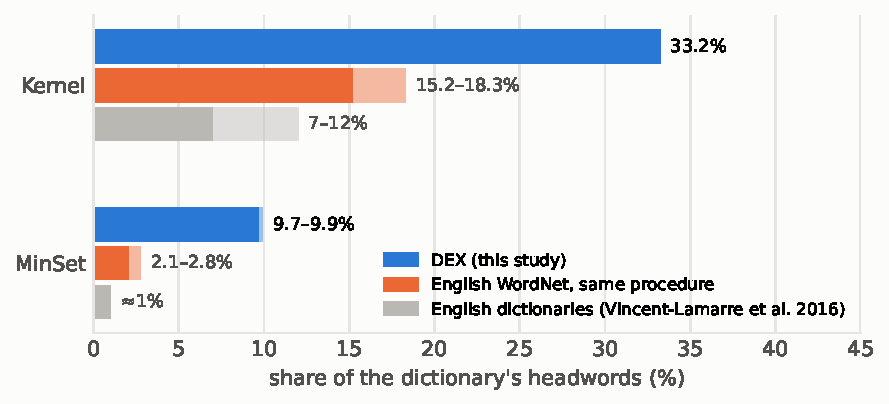
\includegraphics[width=0.72\textwidth]{figures/fig1_size.pdf}
\caption{Proportion of headwords in the Kernel and in the MinSet: the DEX (language-model regime), the English WordNet processed with the same procedure (range over the two regimes without a model) and the English dictionaries studied by Vincent-Lamarre et al. (2016).}
\label{fig:size}
\end{figure}

\begin{figure}[t]
\centering
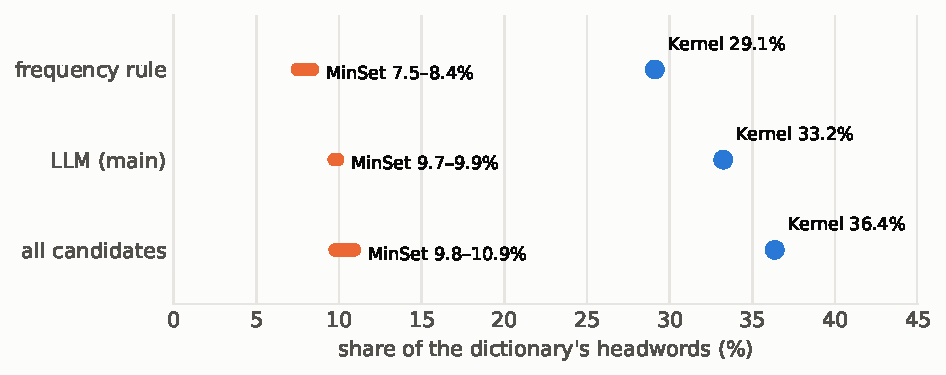
\includegraphics[width=0.72\textwidth]{figures/fig3_robustness.pdf}
\caption{Kernel (dot) and MinSet interval (bar) under the three regimes.}
\label{fig:robust}
\end{figure}

\subsection{Comparison with Other Languages}
The English figures cited above were obtained with a different procedure, so we repeated the analysis under identical conditions for dictionaries of other languages: Princeton WordNet 3.0 \cite{miller1995}, one of the four dictionaries of \newcite{vincentlamarre2016}, and the monolingual Wiktionaries of Romanian and <<X_NLANG>> other languages, in the extraction of \newcite{ylonen2022}. For every dictionary, the vertices are single-word lemmas with a noun, verb, adjective, adverb or numeral entry; the definition of a vertex is the first sense of each of its entries; function words are ignored, as in the study of Vincent-Lamarre et al.; definition tokens are mapped to lemmas with the dictionary's own inflection data; and the two regimes that use no language model are applied. Run through this procedure, the DEX gives a Kernel of <<XD_K>> and a MinSet of <<XD_M>>, close to the values above, so the result does not depend on the procedure. For WordNet the procedure gives a Kernel of <<WN_K>> and a MinSet of <<WN_M>>, somewhat more than the <<VL_WN_K>> and <<VL_WN_M>> reported in the original study. Removing the <<FW_N>> function words of the DEX (prepositions, conjunctions, pronouns, articles and interjections) leaves our main results almost unchanged: the Kernel then contains <<CO_K>> of the content headwords and the MinSet <<CO_M>> (greedy and cycle-packing bounds).

Figure~\ref{fig:crossling} and Table~\ref{tab:crossling} show that the DEX is an outlier. The relative size of the Kernel depends on the size of the dictionary, because large dictionaries contain many rare words that define nothing, whereas the share of the Kernel occupied by the MinSet does not. This share lies between <<X_RATIO>> in the dictionaries of all other languages, Romance languages included, and reaches <<XD_RATIO>> in the DEX. Reciprocally defined pairs are <<X_RLO>> to <<X_RHI>> times more frequent in the DEX than in the other dictionaries. The Romanian Wiktionary has values close to those of the DEX, but it is not independent evidence: <<RW_COPY>> of its first definitions are near-copies of DEX definitions. The large core is therefore a property of the defining practice of the DEX, not of Romance languages.

\begin{figure}[t]
\centering
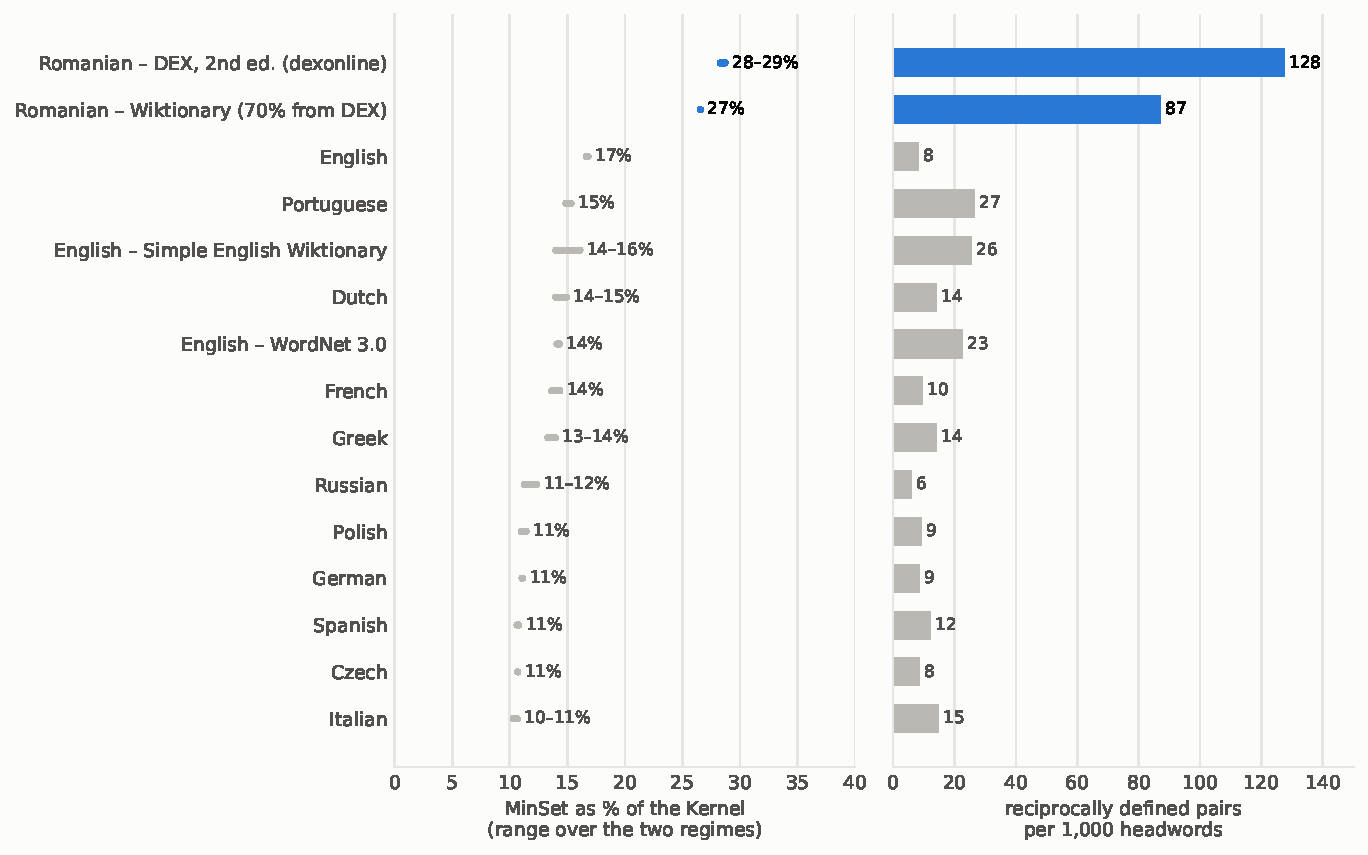
\includegraphics[width=0.9\textwidth]{figures/fig5_crossling.pdf}
\caption{Share of the Kernel occupied by the MinSet (left) and reciprocally defined pairs per 1,000 headwords (right) in dictionaries processed with the same procedure. Romanian dictionaries are shown in blue.}
\label{fig:crossling}
\end{figure}

\begin{table}[t]
\centering
\small
\begin{tabular}{llrrrrr}
\toprule
Language & Dictionary & Headwords & Kernel & MinSet & MinSet/Kernel & Pairs/1,000\\
\midrule
<<TABLE_CROSSLING>>
\bottomrule
\end{tabular}
\caption{Dictionaries processed with the same procedure. Kernel and MinSet are shares of the headwords (ranges over the two regimes without a language model; MinSet: lower bound to upper bound); MinSet/Kernel uses the middle of the MinSet interval. $^{*}$70\% of its first definitions are near-copies of the DEX.}
\label{tab:crossling}
\end{table}

\subsection{Reciprocal Definitions}
The size of the MinSet is explained mainly by reciprocal definition. In the graph, <<PAIRS>> pairs of headwords occur in each other's definitions, for example <<PAIR_EXAMPLES>>. About <<PAIRS_DERIV>> of the pairs share a stem (\ro{masticare}--\ro{masticație}, both `mastication'; \ro{mediere}--\ro{mediație}, both `mediation'), and most of the remaining pairs are synonyms. Each such pair is a cycle of length two, so at least one of its words must belong to every grounding set. Cycles of length two make up <<TWO_CYCLE_SHARE>> of the vertex-disjoint cycles in the packing used for the lower bound. The size of the MinSet therefore follows from the defining practice of the DEX, in which a headword is often defined by a synonym. Romanian lexicographers have discussed the limits of synonymic definition \cite{maranduc2012,sterian2016}. Learner's dictionaries of English, such as the Longman Dictionary of Contemporary English, define their headwords with a restricted defining vocabulary of about 2,000 words \cite{vincentlamarre2016}, which limits cycles of this type. Graur observed the same competition between near-synonyms: he excluded \ro{arbore} `tree' from the fundamental stock because it shares its semantic field with \ro{copac} `tree', \ro{pom} `(fruit) tree' and, regionally, \ro{lemn} `wood' \cite[p.~19]{graur1954}. The language model produces more reciprocal pairs than the most-frequent regime (Table~\ref{tab:regimes}), because it links participles and abstract nouns to their own entries. Examples are \ro{declarat}--\ro{mărturisit} (`declared'--`avowed') and \ro{primejdie}--\ro{risc} (`danger'--`risk').

\subsection{Basic Vocabulary in the Kernel}
A Kernel that results from circular definitions could, in principle, contain any words. We test whether it contains the basic vocabulary by comparing it with the two reference inventories (Table~\ref{tab:inventories}, Figure~\ref{fig:enrich}). The Kernel contains <<SW_K>> of the Swadesh headwords and the MinSet <<SW_M>>, whereas the proportions expected under random selection are <<K_PCT>> and <<M_UB_PCT>>. For Graur's list, the corresponding proportions are <<G_K>> and <<G_M>> ($p < 10^{-200}$, hypergeometric test). The words that Graur considered most certain are more central than those of his two wider groups: <<GC_K>> of them lie in the Kernel and <<GC_M>> in the MinSet, against <<GM_K>> and <<GM_M>> for the middle group and <<GX_K>> and <<GX_M>> for the widest group. The two wider groups differ little from each other.

\begin{table}[t]
\centering
\begin{tabular}{lrrrr}
\toprule
Inventory & Headwords & in Kernel & in MinSet & in Satellites\\
\midrule
<<TABLE_INVENTORIES>>
\midrule
Expected by chance & & <<K_PCT>> & <<M_UB_PCT>> & <<S_PCT>>\\
\bottomrule
\end{tabular}
\caption{Proportion of each reference inventory in the layers of the graph. MinSet: the smallest grounding set found (<<M_UB>> headwords).}
\label{tab:inventories}
\end{table}

\begin{figure}[t]
\centering
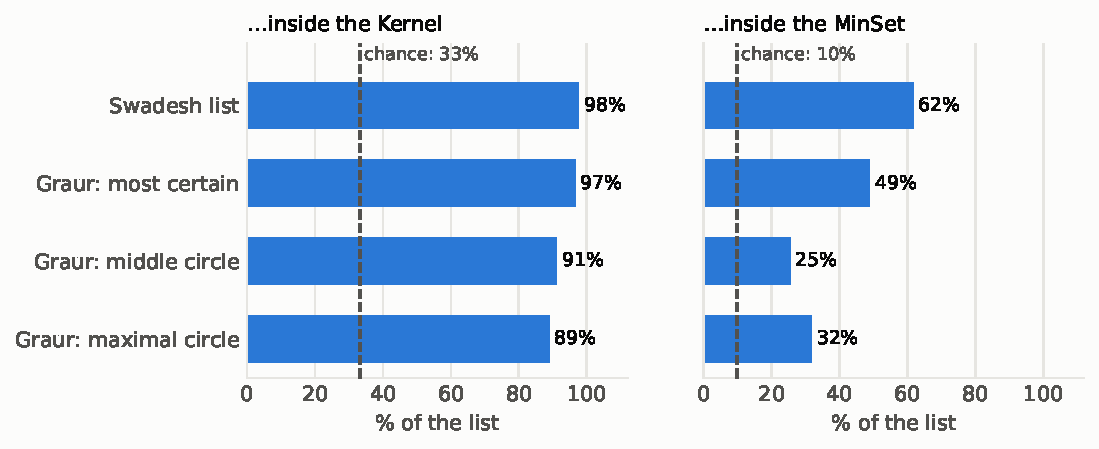
\includegraphics[width=0.82\textwidth]{figures/fig2_enrichment.pdf}
\caption{Proportion of each reference inventory in the Kernel and in the MinSet. The dashed line marks the proportion expected under random selection.}
\label{fig:enrich}
\end{figure}

\subsection{Graur's Examples}
In arguing for his criteria, Graur discussed a number of individual words \cite[pp.~16--25]{graur1954}. Table~\ref{tab:cases} gives their position in the graph. Two of them show how the dictionary and Graur's criteria can diverge. Graur excluded \ro{arbore} `tree' because of its competition with \ro{copac}, \ro{pom} and \ro{lemn}; in the DEX, however, \ro{arbore} is the preferred defining term and occurs in the definitions of <<ARB_O>> headwords, against <<COP_O>> for \ro{copac}. Graur placed \ro{femeie} `woman' only in his widest group, because its modern sense was recent and competed with \ro{nevastă} `wife' and \ro{muiere} `woman (popular)'; in the DEX, \ro{femeie} occurs in <<FEM_O>> definitions and belongs to the MinSet. The graph records how lexicographers use a word in definitions, whereas Graur's criteria concern the history of a word and its use by speakers, and the two can lead to different rankings.

\begin{table}[t]
\centering
\begin{tabular}{lllll}
\toprule
Word & Gloss & Graur (1954) & Graph layer & Used in definitions of\\
\midrule
<<TABLE_CASES>>
\bottomrule
\end{tabular}
\caption{Position in the DEX graph of words discussed by Graur (1954).}
\label{tab:cases}
\end{table}

\subsection{The Most Frequent Defining Words}
Only <<G_OUT>> of Graur's words lie outside the Kernel, among them <<G_OUT_EXAMPLES>>. Most of them belong to the vocabulary of traditional rural life, and the DEX defines them without using them in the definitions of other headwords. The words that the DEX uses most often in definitions form a different set. To compare sets of equal size, we take the 1,419 headwords that occur in the largest number of definitions. Only <<TOP_OVERLAP>> of them belong to Graur's list, and the two sets differ in origin (Figure~\ref{fig:etym}). With the same etymological classification, Graur's list is <<ET_G_LAT>> Latin and <<ET_G_SL>> Slavic, whereas the most frequent defining words are <<ET_T_FR>> French, <<ET_T_LAT>> Latin and <<ET_T_SL>> Slavic. Table~\ref{tab:top} lists the 30 content words used most often in definitions. Most of them are learned or abstract terms, such as \ro{acțiune} `action', \ro{rezultat} `result' and \ro{persoană} `person'.

\begin{table}[t]
\centering
\small
\begin{tabular}{lr|lr|lr}
\toprule
Word & N & Word & N & Word & N\\
\midrule
<<TABLE_TOP>>
\bottomrule
\end{tabular}
\caption{The 30 content words used most often in DEX definitions; N is the number of headwords whose definition contains the word. Words in Graur's list are marked with $^{G}$.}
\label{tab:top}
\end{table}

\begin{figure}[t]
\centering
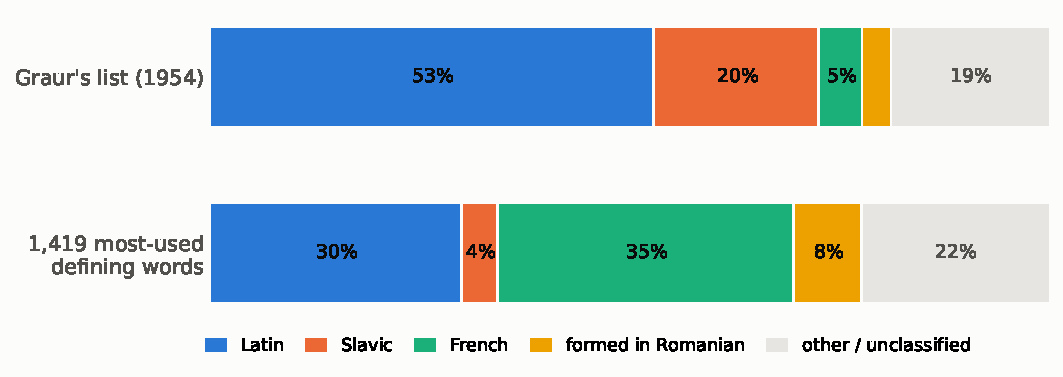
\includegraphics[width=0.82\textwidth]{figures/fig4_etymology.pdf}
\caption{Origin of Graur's words and of the 1,419 words most used in DEX definitions, both classified from DEX etymologies.}
\label{fig:etym}
\end{figure}

\section{Discussion}
\subsection{Answers to the Research Questions}
(Q1) The DEX is considerably more circular than the dictionaries of other languages studied so far. About one third of its headwords belong to the Kernel, and about one tenth must be known in advance for all the others to be learnable from first-sense definitions. Dictionaries of <<X_NLANG>> other languages processed in the same way, Romance languages included, need much smaller grounding sets (<<X_M>> of their headwords). (Q2) The difference is explained mainly by the definition of headwords through synonyms and derivatives: cycles of length two account for <<TWO_CYCLE_SHARE>> of the disjoint cycles that determine the lower bound. (Q3) The Kernel contains almost all the basic vocabulary identified by two independent inventories, and Graur's most certain words are the most central of his list. The Kernel thus combines two groups of words: the inherited basic vocabulary described by Graur, and a group of learned, mostly French, abstract words that the DEX uses as its defining vocabulary.

\subsection{Uses of the Results}
The results and the released data have four direct uses. First, in lexicographic revision, the list of reciprocally defined pairs shows where the DEX defines a word only through a synonym. Some circularity is unavoidable in any dictionary, but the list allows editors to examine each case and to decide where an analytical definition is needed; new or revised definitions can be checked in the same way before publication. Second, the Kernel and the MinSet, combined with corpus frequency, give an empirical starting point for a restricted defining vocabulary of Romanian, of the kind used in learner's dictionaries, and for the selection of vocabulary in teaching Romanian as a foreign language. Third, for natural language processing, the graph and its layers are a resource for tasks based on dictionary definitions, such as the detection of semantic primitives \cite{pichardo2017,kostiuk2023} or the evaluation of the definitions that language models produce for Romanian words. Fourth, for the history of Romanian linguistics, the comparison tests Graur's list with data that were not available to him, and it can be repeated for later inventories of basic vocabulary.

\section{Limitations}
The study analyses one Romanian dictionary in one digitised edition, from which a few entries are missing (e.g.\ \ro{umbră} `shadow'), and compares it with Wiktionaries, whose editorial practice differs from that of an academic dictionary. The only other Romanian dictionary available to us, the Romanian Wiktionary, largely copies the DEX, so it remains open whether the large core is specific to the DEX or common to Romanian lexicography. Using only the first sense and merging homonyms simplifies the graph, as in previous work, and the results may change when all senses are included. The language model is not free of errors: it agrees with a stronger model on <<AGREE_CONTENT>> of the content-word decisions, and agreement between two models does not guarantee correctness. For this reason all results are given under three regimes, which lead to the same conclusions. <<MINSET_LIMITATION>> The etymological classifier leaves part of the vocabulary unclassified. The comparison with Graur depends on our transcription and lemma mapping, which we checked against his published totals. Psycholinguistic data such as age of acquisition, which \newcite{vincentlamarre2016} used for English, are not available for Romanian at this scale, so we could not test whether Kernel words are acquired earlier.

\section{Data and Code Availability}
The code, the derived data and the figures are available at \url{https://github.com/ovladon/hidden-core-romanian} under the GNU General Public License, version 3, the licence of the dexonline data from which they are derived. The repository contains the dictionary graph as a list of arcs (one line per pair of defining word and defined headword), the layer of each headword (MinSet, Core, Satellite or outside the Kernel), the list of reciprocally defined pairs, the choices of the language model for every ambiguous token, and the numbers reported in this paper. The documentation lists the commands that reproduce every number from the public dexonline database dump; the language model is needed only to recompute the disambiguation, whose results are included. The script \texttt{latent\_structure.py} applies the graph analysis to any dictionary supplied as a list of arcs, so the method can be used for other Romanian dictionaries, for instance later editions of the DEX or the DLR (\ro{Dicționarul limbii române}, The Dictionary of the Romanian Language), and for other languages. The scripts of the cross-linguistic comparison are included; the Wiktionary data (CC BY-SA) are downloaded by a script from the source and are not redistributed. Our transcription of Graur's list is not distributed, for copyright reasons.

\section{Conclusion}
We have presented the first analysis of the latent structure of a Romanian explanatory dictionary. In the DEX, one third of the headwords form a Kernel from which all the other headwords can be defined, and about one tenth must be known in advance for the whole dictionary to be learnable from first-sense definitions. Dictionaries of <<X_NLANG>> other languages processed in the same way need only <<X_M>> of their headwords. The main cause is the frequent definition of a word by a synonym or a derivative. The Kernel contains almost all the words of the Swadesh list and of Graur's fundamental lexical stock, and the words that Graur considered most certain are the most central of his list. The words used most often in definitions, in contrast, are mainly learned French loanwords. The language model performs a narrow task whose output can be inspected, and the conclusions remain the same when it is replaced by simple rules. Further work will include all senses of each entry and Romanian dictionaries independent of the DEX.

\section*{AI Use Statement}
A large language model is part of the method described in this paper (Section~3.3): Claude Haiku~4.5 \cite{anthropic_models} selected the intended headword for each ambiguous word form in a definition, and Claude Opus~5 was used to estimate the reliability of these selections. In addition, an AI assistant (Claude, Anthropic) was used under the authors' direction to help write the analysis code, to search the literature and to draft and edit the text and the abstract. The authors reviewed all generated code, numbers and text, verified them against the data and corrected them, and take full responsibility for the content of the paper.

\bibliographystyle{consilr}
\bibliography{references}
\end{document}
